\subsection{Unsupervised Learning Algorithms}
\label{sec:unsupervised}
When Hart initially proposed energy disaggregation,
the problem was tailor made for unsupervised learning methods~\cite{hart1992} because
the exact information of individual circuits or devices
is unknown.
In recent times, unsupervised disaggregation has emerged as a hotbed for research. 
Clustering~\cite{gonccalves2011unsupervised} is used to group similar events. Different approaches such as 
HMM~\cite{kim2011unsupervised,kolter2012aistat,parson2012nonintrusive} and temporal mining~\cite{shao2012temporal} have been applied. 
Clustering-based disaggregation algorithms are designed under the following assumption:
{\em Events and features generated by a single device will be clustered together.}
These techniques apply a known clustering algorithm to the data set and group events generated by a device.
While clustering techniques have been designed with no knowledge on the number of devices, some unsupervised learning methods also assume that the number of devices is also known.
 
\subsubsection{Hierarchical clustering-based}
Gonccalves et al. proposed a method that disaggregates devices without a-priori knowledge of the total number of devices ~\cite{gonccalves2011unsupervised}. 
As the first step, in order to extract the real and reactive power features, blind source separation~\cite{lee1999blindsource} is used. 
In the second step, hierarchical agglomerative clustering of real and reactive power is used to cluster the on and off events.
The greedy matching pursuit (MP), which is a direct implementation of Hart's intuition,
is calculated in terms of Euclidian distance
$([P_t,Q_t]-[P_{closest},Q_{closest}])$.

\textbf{Computational Complexity}
\cite{gonccalves2011unsupervised} only studies disaggregating devices with 
on and off events. 
In this study, the real power and reactive power are used. 
The computational cost of the measurement of pair-wise distances 
is $O(T^2)$, where $T$ is the number of points in aggregated time series. 
For agglomerative clustering, 
the computational cost of unsupervised 
disaggregation is $O(T^2)logT$~\cite{jain1999data}. 

\textbf{Advantages and Disadvantages of Clustering-based Unsupervised Learning Techniques}

The \textit{advantages} of clustering-based unsupervised techniques are as follows:
\begin{enumerate}
\item It is easy to set up the model even if the number of devices is 
not known.
%\item The computational cost is not high. 
\end{enumerate}

The \textit{disadvantages} of clustering-based techniques are as below:
\begin{enumerate}
\item Clustering-based technique may incorrectly group the devices with same power levels. 
\item These techniques are applied to devices with two states, on and off, but not applicable 
to devices with multiple states.  
\end{enumerate}

\subsubsection{FHMM-based}
The factorial hidden semi-Markov model (FHMM) is a relatively new unsupervised energy disaggregation approach. 
It assumes that we know the number of devices inside a building 
and the power usage of the entire house is available. 
Kim et al proposes an FHMM technique and FHMM~\cite{kim2011unsupervised} to disaggregate devices in the manner described below. 
As shown in Figure~\ref{fig_fhmm} (a),
FHMM uses multiple HMMs to model
the status of each device. 
The aggregated power at a specific time is given by adding the values produced by the HMM corresponding to each device.
%\begin{figure}[ht]
%\centering
%\includegraphics[width=3in]{figs/fhmm_kim2010unsupervised.pdf}
%\caption{Graph Model of FHMM with $N$ Devices.}
%\label{fig_fhmm_kim2010unsupervised}
%5\end{figure}

\begin{figure*}[ht]
	\centering{
    \begin{tabular}{cc}	
    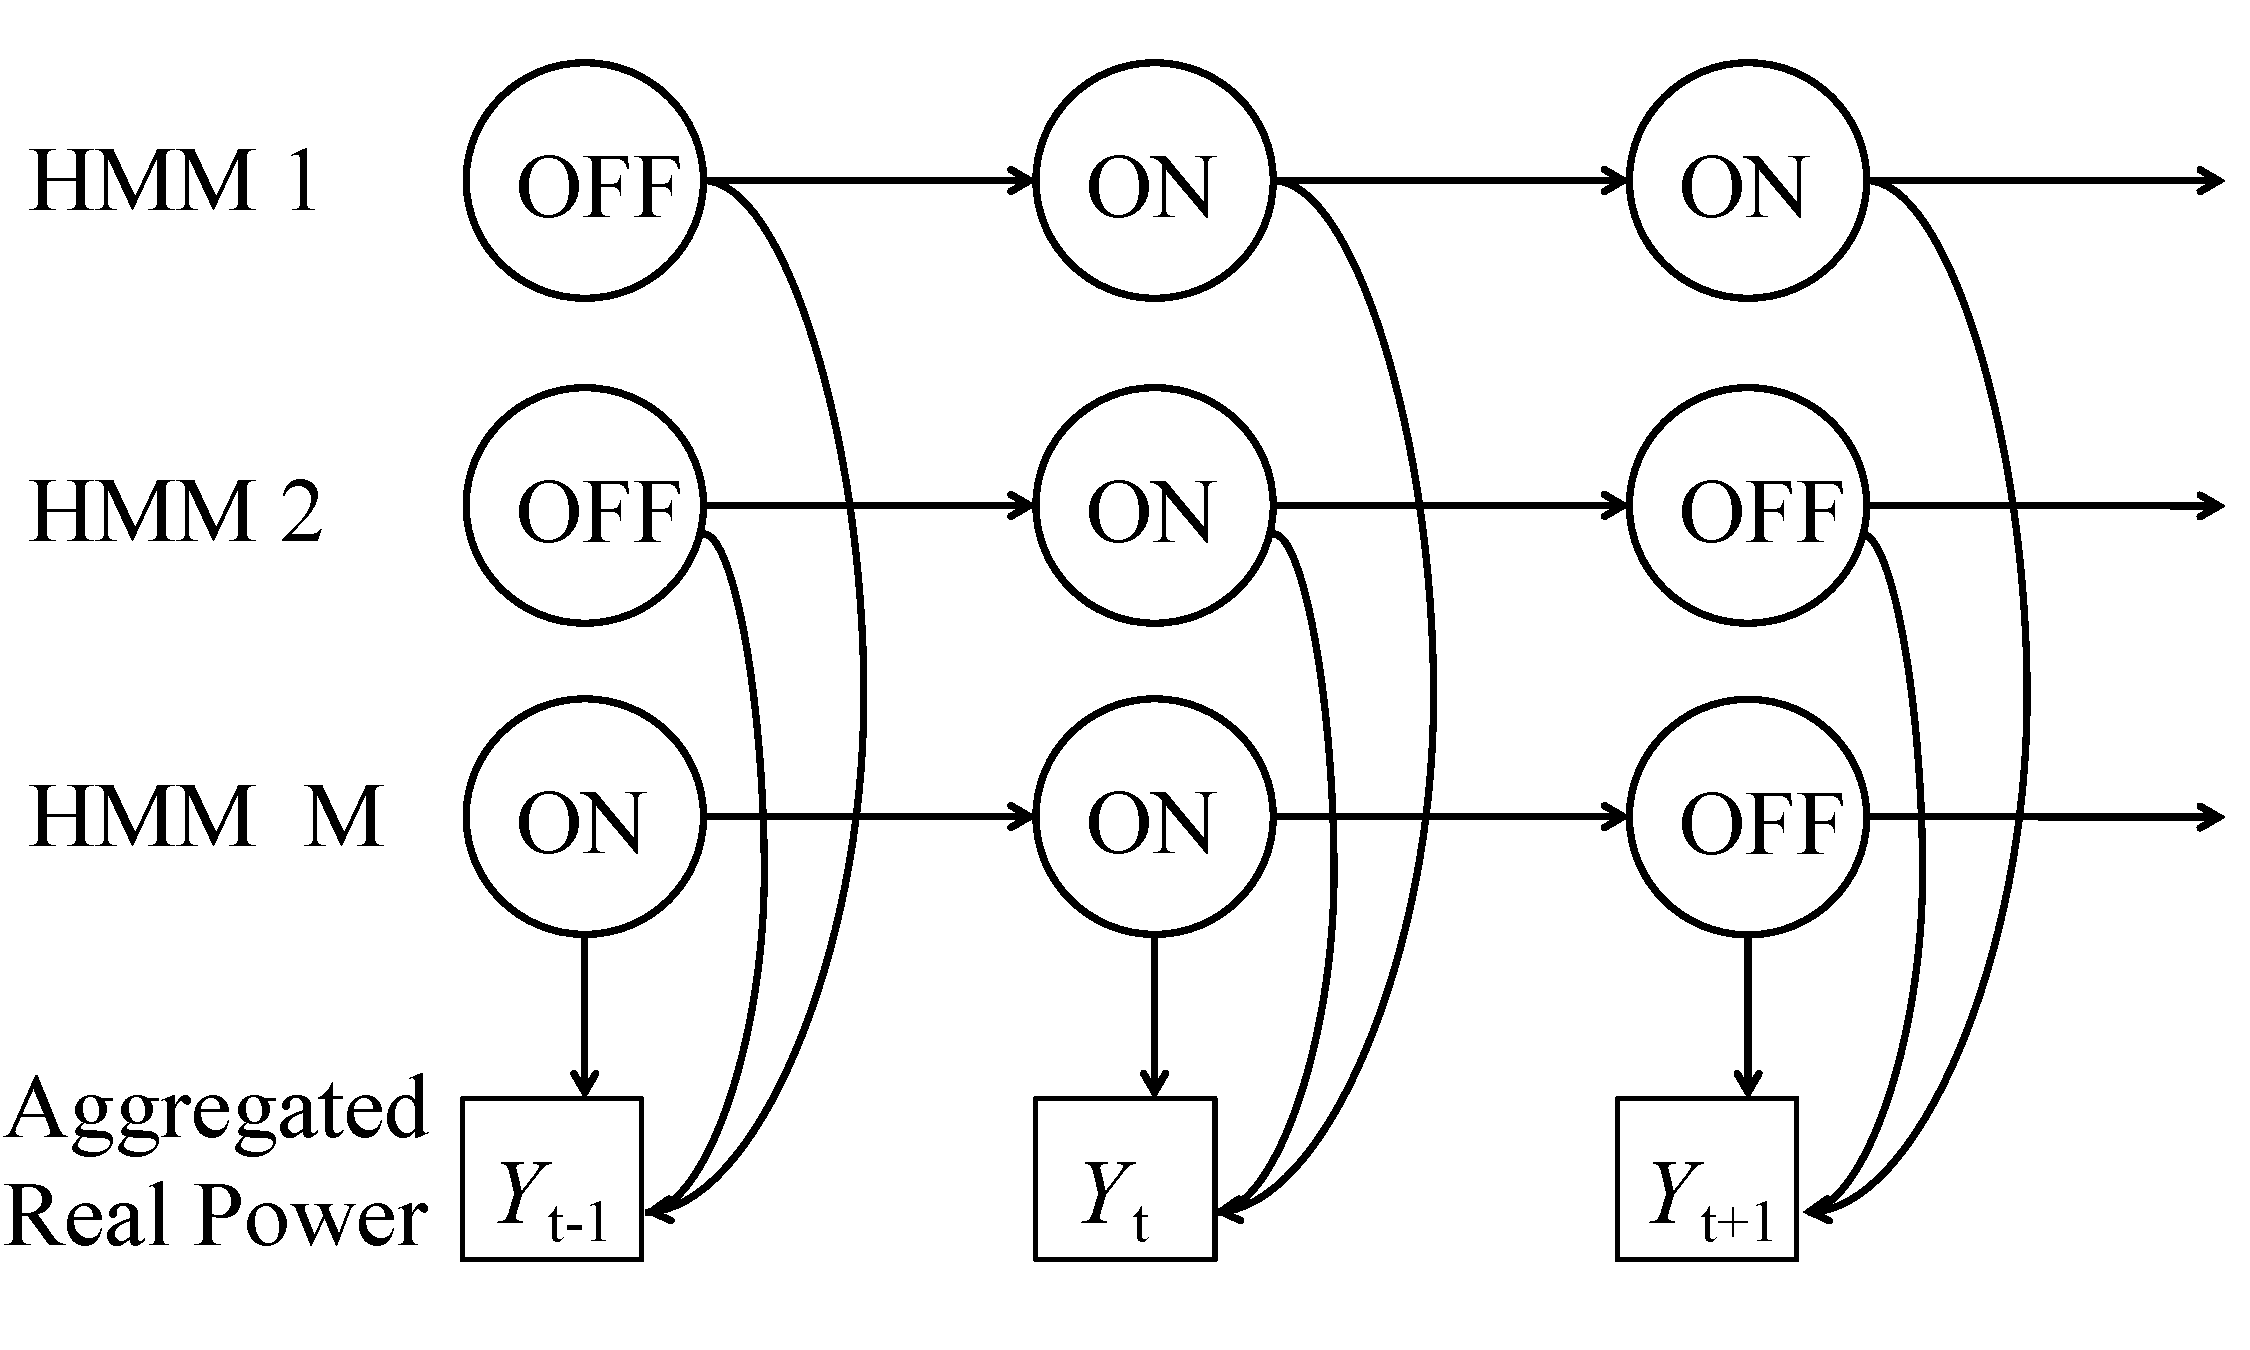
\includegraphics[width=0.5\textwidth]{figs/fhmm.pdf}\hspace{1em}&
	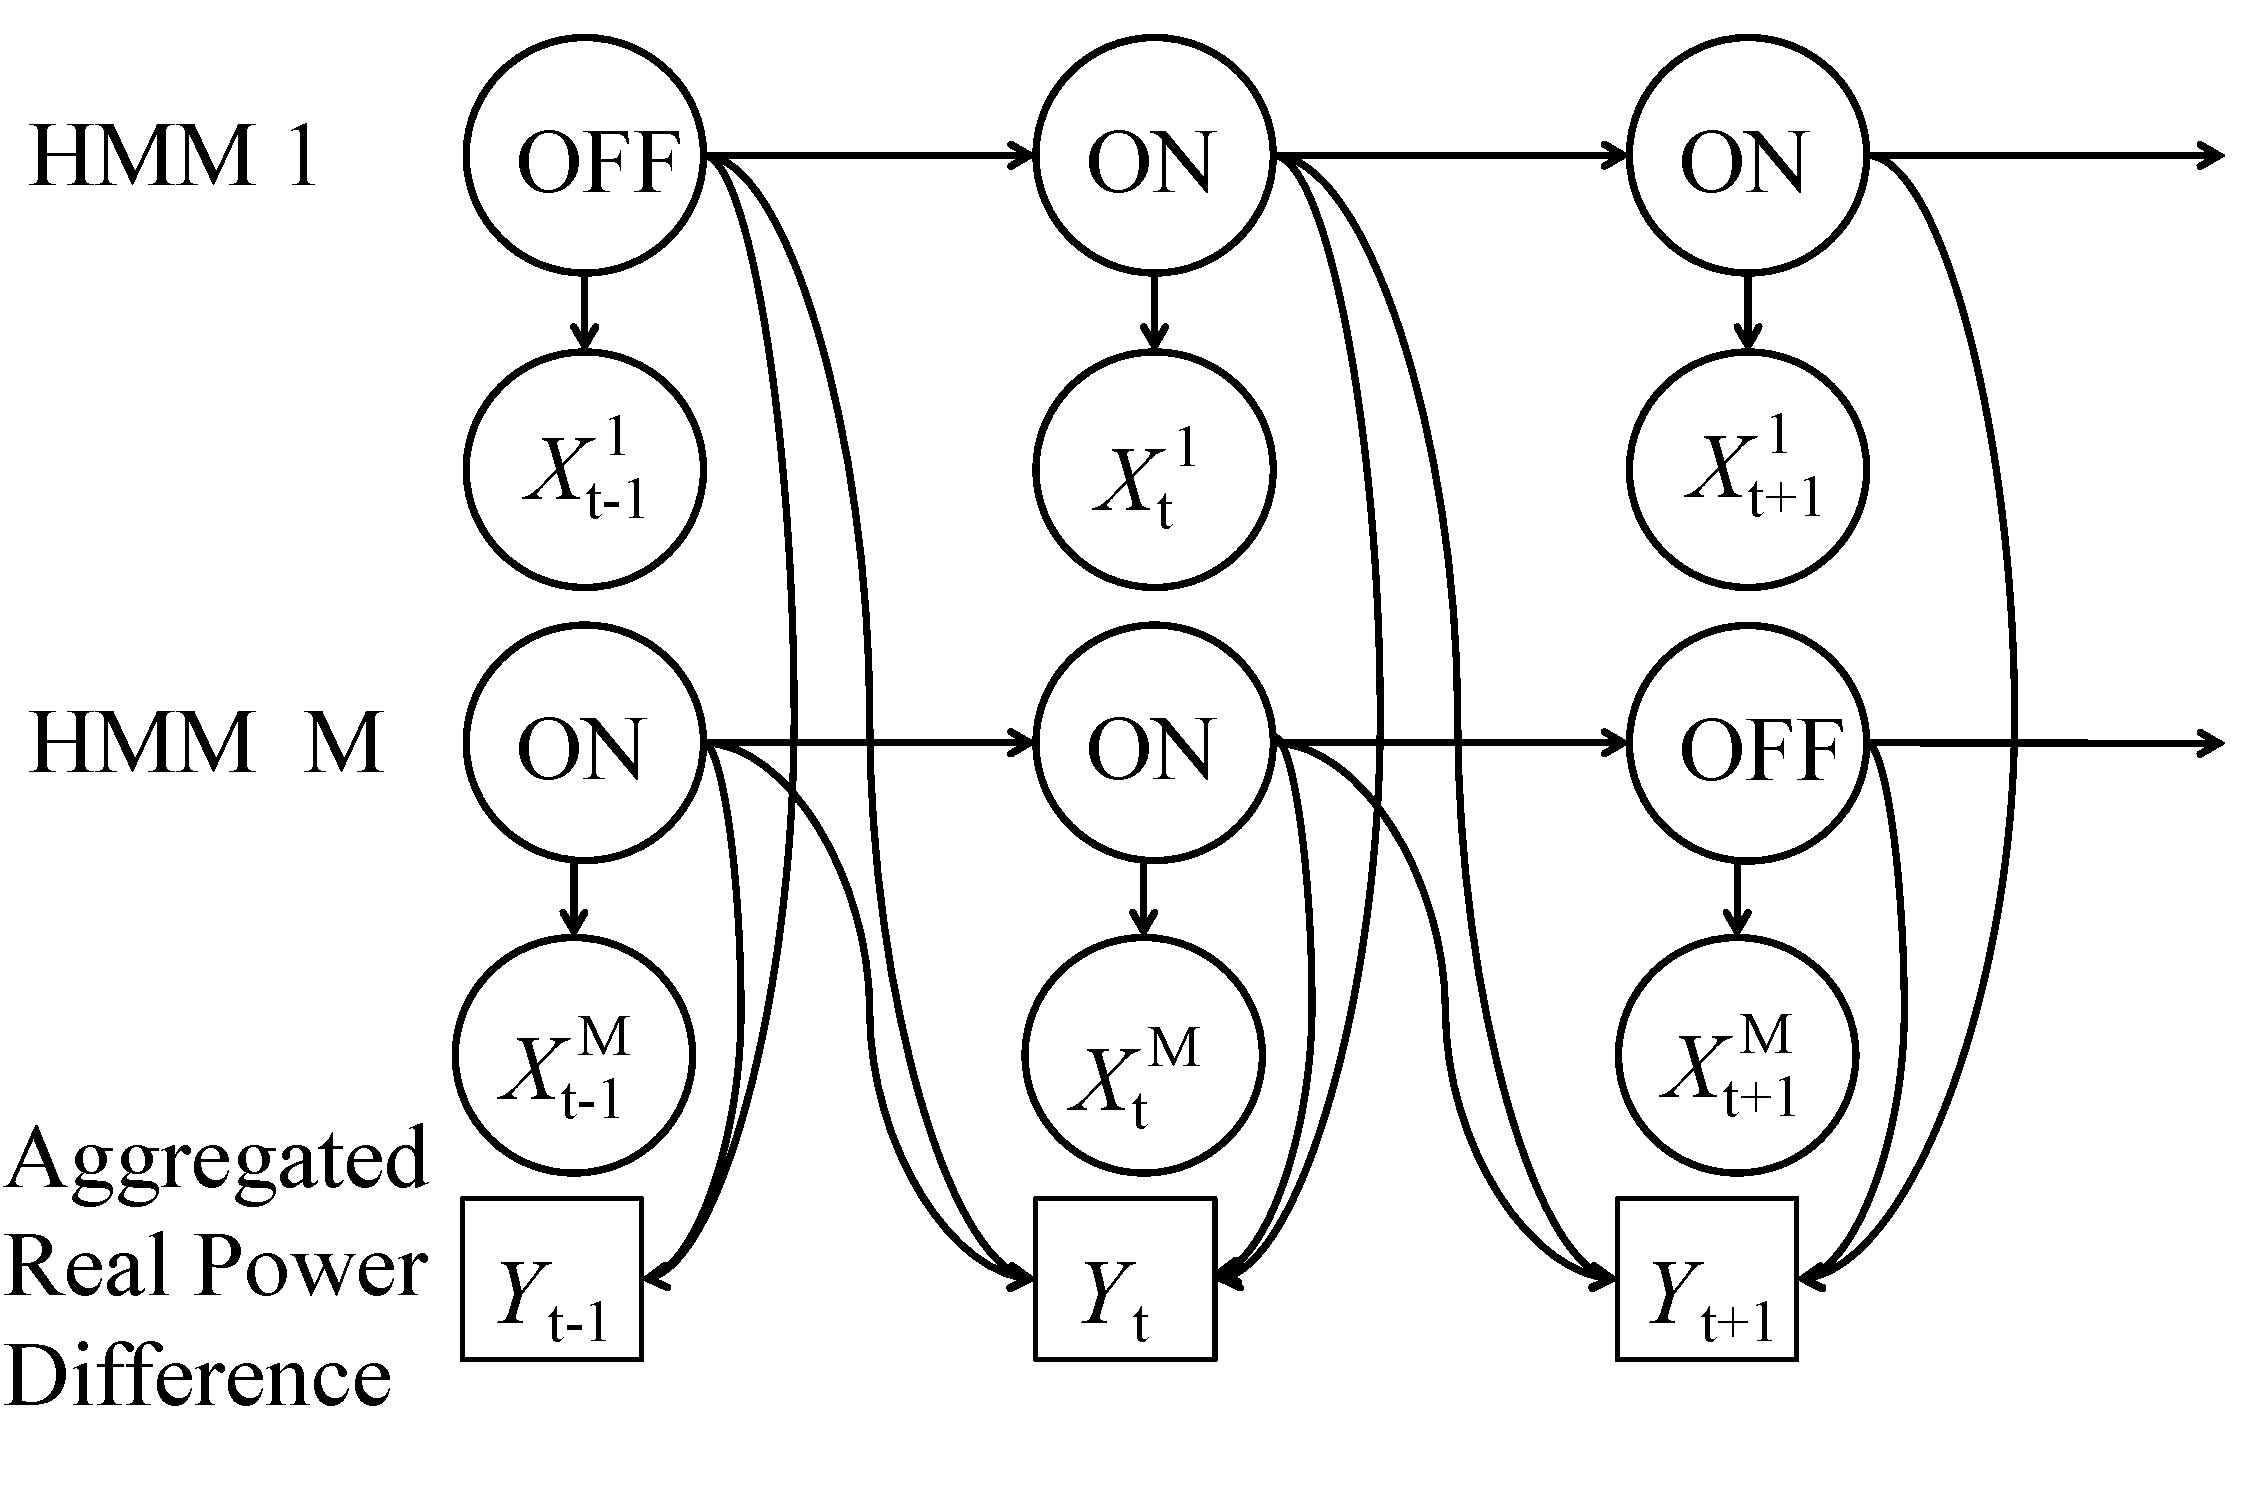
\includegraphics[width=0.5\textwidth]{figs/difference_fhmm.pdf}\tabularnewline
   (a) & (b) \tabularnewline
    \end{tabular}
    }
	\caption{ Graphical model with $M$ devices. (a) FHMM and (b) Difference FHMM.}
	\label{fig_fhmm}
\end{figure*}

FHMM and constraint FHMM
extend FHMM by incorporating the time duration for which the device is turned on, the
correlation between various devices, and the usage time of each device. 

We form the FHMM by calculating the initial probability $\phi_{in}(y,x|\Theta)$,
emission probability $\phi_{e}(y,x|\Theta)$, and
transition probability $\phi_{t}(y,x|\Theta)$,
where $\Theta$ is the parameter set.
The product of these three probability is given in Equation (\ref{eq_fhmm}).
\begin{equation}
\label{eq_fhmm}
P(y,x|\Theta)= \phi_{in}(y,x|\Theta) \cdot \phi_{e}(y,x|\Theta) \cdot \phi_{t}(y,x|\Theta)
\end{equation}
By maximizing Equation (\ref{eq_fhmm_em}) with the EM algorithm,
we can derive the HMM which represents the device. 
\begin{equation}
\label{eq_fhmm_em}
\phi(\Theta,\Theta^\prime)= \sum_x P(y,x|\Theta^\prime) log P(y,x|\Theta)
\end{equation}
where $\Theta^\prime $ and $\Theta$ represent the previous and current
iteration parameter set of the EM algorithm.

A variant of FHMM is the Additive Factorial Approximate Maximum a Posterior (AFAMAP)~\cite{kolter2012aistat}.
It is a mixture of the additive factorial model and
difference FHMM model.
The box diagram of AFAMAP is as Figure~\ref{fig_AFAMAP_boxDiagram}.
\begin{figure}[h]
\centering
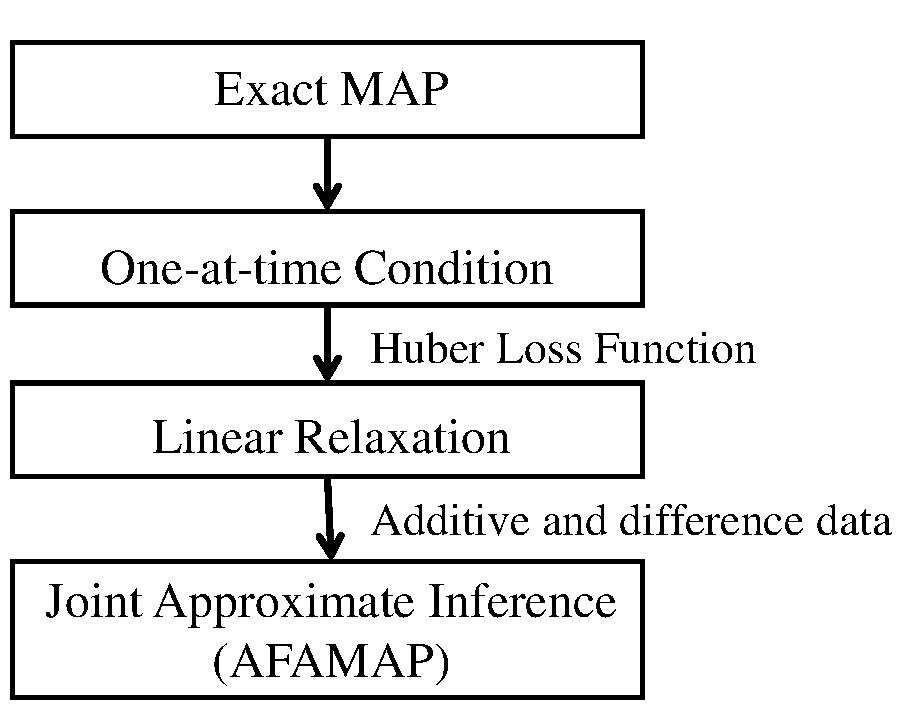
\includegraphics[width=2.5 in]{figs/AFAMAP_Boxdiagram.pdf}
\caption{AFAMAP Flowchart.}
\label{fig_AFAMAP_boxDiagram}
\end{figure}


The disaggregation procedure comprises of the following four steps. 
Initially, the MAP is proposed and
priors are defined as a Laplace prior given in Equation (\ref{eq_afamapPrior}).
\begin{equation}
\label{eq_afamapPrior}
\begin{aligned}
p(z_{1:T})= \frac{1}{Z(\theta,T)}exp\{-\theta \sum_{t=1}^{T-1} \lVert z_{t+1}-z_{t-1}\rVert_1\} \\
p(\Delta z_{1:T})=\frac{1}{Z(\theta,T)}exp\{-\theta \sum_{t=1}^{T}\lVert \Delta z_t \rVert_1\}
\end{aligned}
\end{equation}
where $z_t$ is a introduced signal, and $\Delta z_t = z_{t+1}-z_{t-1}$.
Thus the posterior of additive and difference model turns into a Gaussian distribution 
separately. 
\begin{equation}
\begin{aligned}
y_t|x_t^{(1:M)},z_t\sim \mathcal{N}(\sum_{m=1}^{M}\mu_{x_t^{(m)}}^{(m)}+\Sigma^{1/2}{z_t},\Sigma)\\
\Delta y_t|x_{t-1}^{(1:M)},\Delta z_t\sim \mathcal{N}(\sum_{m=1}^{M}\Delta \mu^{(m)}_{x_t^{(m)},x_{t-1}^{(m)}}+\Sigma^{1/2}\Delta z_t,\Sigma)\\
\end{aligned}
\end{equation}
where $\mu_j^m$ is the mean of the $m$th HMM for the state $j$, 
$x_t^{(m)} \in {1,...,S_m}$ denotes the state of the $m$th HMM at time $t$. 

Then in the second step, the once-at-a-time constraints are added as in Equation (\ref{eq_onceatime}) to limit that at any given time, 
only one device is turned on or off. 
\begin{equation}
\label{eq_onceatime}
\mathcal{O} = {\mathcal{Q}: \sum_{m,j,k \neq j} Q(x_{t-1}^{(m)},x_t^{(m)})_{j,k}\leq 1}
\end{equation}
Till this step, to solve the MAP, the computation cost is very high. 
In order to get a resolved solution, in the third step, the Huber loss function is employed to perform optimization by linear relaxation. 
\begin{equation}
\begin{aligned}
D(y,\theta)= \min_{z}\{\lVert y-z \rVert_2^2+ \theta \lVert z \rVert_1\} \\
= \sum_{\ell=1}^{n}\min\{\frac{1}{2}y_{\ell}^2,max\{\theta|y_{\ell}|-\frac{\theta^2}{2}, \frac{\theta^2}{2}\}\}
\end{aligned}
\end{equation}

Thus disaggregation is converted to a joint approximate inference AFAMAP problem.  
It's a convex quadratic program which can be solved by classical optimization algorithms.
Then with aggregated data as input, we can get the $M$ number of HMMs corresponding to $M$ devices. 

Another variant of FHMM was proposed in~\cite{parson2012nonintrusive}. 
The difference FHMM is shown as Figure~\ref{fig_fhmm} (b). 
This method assumes that we know the labels of each device, thus meaning that the number of devices and device names are known. 
However, the power usage of each device is unknown. 
In the first step, the aggregated data is 
trained to get the features of each device. 
Since this training process only uses the aggregated data, we classify this approach into unsupervised disaggregation. 
During the procedure, 
the features are repeatedly deleted. 
Then more device features are gradually identified. 
In the next step, the appliance behavior like peaks arising from device being turned on or the power demand of the device, 
obtained from the previous step is used as a prior for the difference FHMM. Then the EM algorithm is used to evaluate the likelihood of whether the profile is of a certain device type.
\begin{displaymath}
accept(y_{t},...,y_{t+w}|\hat{\theta})= \left \{ \begin{array} {ll}
true & \textrm{if $\ln\mathcal{L} > \mathcal{D}$ } \\
false & \textrm{otherwise} \end{array} \right.
\end{displaymath}
where $y_t,...,y_{t+w}$ represents the data in a window size $w$
beginning from index $t$ to $t+w$, $\mathcal{L}$ denotes the
likelihood given the prior parameter $\hat{\theta}$,
$\mathcal{D}$ is the predefined likelihood threshold.
In the final step, all these devices are disaggregated by an extended viterbi algorithm. 

Further,~\cite{huang2013designing} uses HMM for electric heat usage disaggregation. %(maybe more explanation.?)
HMM and AFAMAP are also run by additional applications~\cite{lukaszewski2013methods}. 

\textbf{Computational Complexity}
The computational cost varies for these two kinds of unsupervised learning 
approaches.
Generally the computational cost of FHMM and its variants is exponential in 
the number of latent chains.  
Theoretically, the computational complexity is 
$O(MS^{2K})$, where $M$ devices correspond to $M$ chains, 
each device has $S$ states, and $K$ latent variables~\cite{bishop2006pattern}. 
It's hard to obtain the direct solution theoretically. 
Therefore Gibbs sampling is applied to the first 
FHMM solution~\cite{kim2011unsupervised}. 
Later in the AFAMAP, QP problem techniques are used in the solution.
In another variant of difference FHMM~\cite{parson2012nonintrusive}, 
the viterbi algorithm is applied. 

\textbf{Advantages and Disadvantages of FHMM-based Unsupervised Techniques}
%The advantages and disadvantages of FHMM based unsupervised learning techniques are as follows:

The \textit{advantages} of FHMM-based unsupervised learning techniques are as follows:
\begin{enumerate}
\item It's the first formally proposed unsupervised learning approach.
\item It's solvable by introducing MCMC or converting it to an optimization problem.
\end{enumerate}

The \textit{disadvantages} of FHMM-based techniques are as below:
\begin{enumerate}
\item The computational cost is high. 
\item The parameters obtained from the MCMC approach are not easy to estimate. 
\end{enumerate}

\subsubsection{Temporal mining-based}

A lightweight time series motif mining method~\cite{shao2012temporal}
is proposed to identify devices rapidly.
In this approach, a motif which represents a multiple-state device,
is discovered in a time series of aggregated real power. 
Figure~\ref{fig_motifSample} illustrates how a motif is found.
Non-overlap search for a single episode explains
multiple-state changes for a device. A device turns on, then
its state changes to another state, until it turns off. 
This episode
corresponds to a complete running cycle of a device. A
device may include multiple episodes.
Between any two episodes, overlap does exist. For example,
the second instance of Episode1 overlaps with the first
instance of Episode 2. The overlap between episodes explains
the operations of several devices. We regard Episode
1 as device A and Episode 2 as device B. When device
B turns on for the first time, before it turns off, device A
turns on for the second time then turns off, then device B
turns off.
\begin{figure}[ht]
\centering
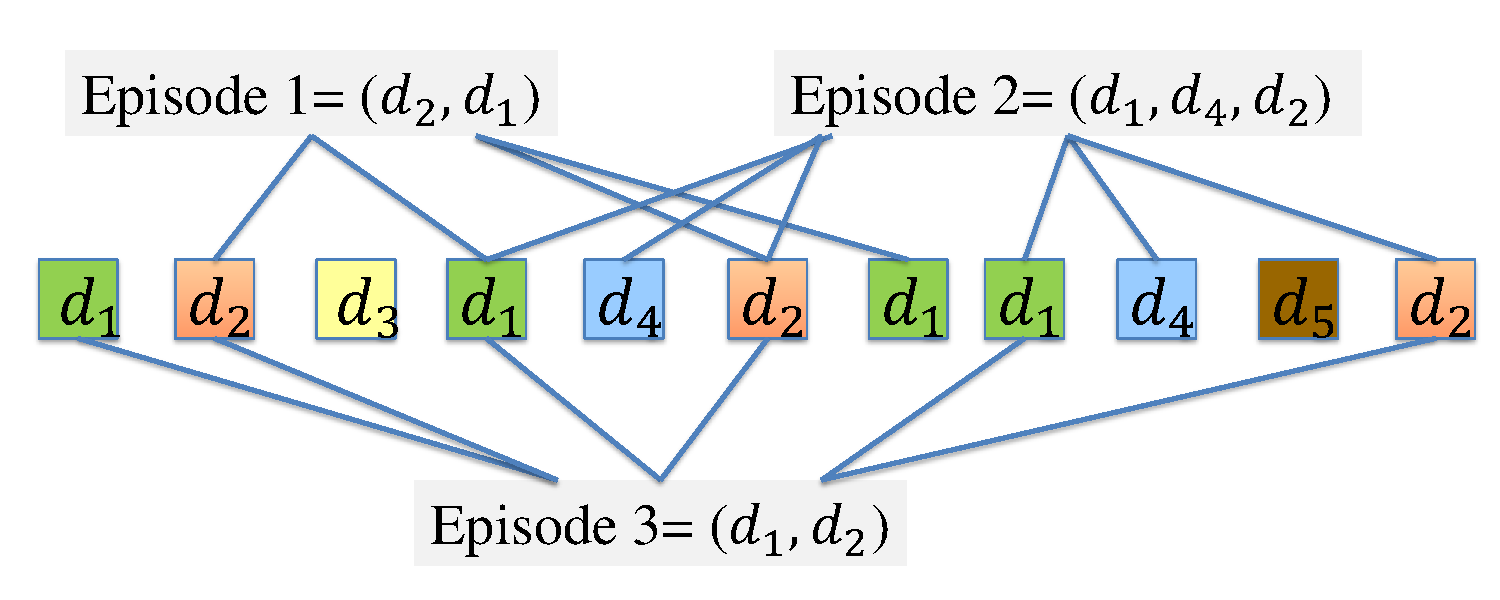
\includegraphics[width=3in]{figs/motifSample.pdf}
\caption{Motif Mining Example (\cite{shao2012temporal}). }
\label{fig_motifSample}
\end{figure}
Also, it can integrate with AFAMAP~\cite{kolter2012aistat}.
The output of motif mining can be used as the input of
AFAMAP.

\textbf{Computational Complexity}
Assume $m$ is
the number of power levels in the `diffs' data. Then the computational complexity of
DPGMM is $O(mnd^2+md^3)$, where $n$ is the number of points in diffs data,
and $d$ is the number of feature dimensions (e.g.,  time, date).
The computational complexity
for the episode generation step is $(p-1)O(m^2)$, where $p$ is the
maximal
episodes length. Since $p$, which is 3, and $m$, which is 14 or 27, are small,
we apply a brute force approach. The worst-case time complexity of the motif
mining algorithm is $O(msq)$, where $q$ is number of candidate episodes, and
$s$ is the size of the episode.

\textbf{Advantages and Disadvantages of Temporal Mining-based Unsupervised Techniques}
%The advantages and disadvantages of factorial-HMM based unsupervised learning techniques are as follows:

The \textit{advantages} of temporal mining-based techniques are as follows:
\begin{enumerate}
\item It's a lightweight approach. 
\item The disaggregation results are comparable to the results from 
complex models. 
\item It's applied to multi-state devices. 
\item It can capture device disaggregation even from commercial buildings. 
\end{enumerate}


The \textit{disadvantages} of temporal mining-based techniques are as below:
\begin{enumerate}
\item The smoothing parameter is not adjusted automatically. 
\item The problem is not formally proposed.  
\end{enumerate}

\iffalse
\subsubsection{Nonnegative matrix factor 2-D deconvolution}
A shift-invariant sparse coding model is adopted for single channel blind source separation 
in the area of signal processing~\cite{blumensath2005shift} although 
the energy dataset has not been tested so far. 
At first, the single blind source separation is formulated as a linear mixture model incorporating 
two constraints, namely sparseness and non-negativity. 
\begin{equation}
Y= XS+\epsilon
\end{equation}
Where $Y$ is the aggregated data, 
$X$ represents the feature, 
$S$ is the power level, i.e. the scalar of feature, 
and $\epsilon$ is a vector of i.i.d. Gaussian noise. 

Then three sub-problems are addressed. First is to learn the model parameters. 
The second is to infer the model states and the last is to discover the features. 
In the first step, the single source separation problem is formulated as a Bayesian problem. 
Since there are i.i.d. noise conforming to Gaussian distribution, 
$p(\epsilon) \sim N(0, \sigma_{\epsilon}I)$, 
the Gaussian likelihood is defined as $p(y|X, S) \sim N(XS, \sigma_{\epsilon}I)$. 
Take the gradient, 
$p({Y}|X) \propto \int p(Y|X, S) p(S) dS$, where $p(S)$ is the prior. 
To maximize the marginal likelihood, 
a stochastic gradient descent optimization approach is proposed by 
integrating with Monte Carlo approach. 
The features are discovered by clustering approach. 

\subsubsection{ICA or PCA-based}
\cite{davies2007source} uses ICA for signal source separation although 
the energy datasets haven't been tested yet. 

\cite{smaragdis2006probabilistic} uses the PLCA for single source separation based on 
both the time and frequency domain.
The features can be learned unsupervised by EM algorithms.
\fi

\subsubsection{Probabilistic graph-based}
Besides HMM, another probabilistic graph model was proposed by~\cite{kelly2012disaggregating}. 
The model is composed of three layers. The component layer forms the the bottom most layer, 
the second layer comprises of a probabilistic graph model that captures appliances, and
finally the top-most later us an inter-appliance layer. 
So far, this approach has not implemented in detail. 


\subsection{Semi-supervised Learning Algorithms}
Semi-supervised algorithms assume that the feature for each device, such as the power levels of 
the device is already known.
Instead of extracting features from the training data, 
it utilizes the features from the aggregated data using unsupervised algorithms. 
Then these features are used to predict devices from the test data. 

Assumption: \textit{The features are clustered based on the device i.e. all the known features
that characterize a device are grouped together.} 

\subsubsection{Clustering-based} 
Lam et al. initially propose to utilize voltage-current (V-I) trajectory of appliance as 
a feature to perform clustering~\cite{lam2007novel}.  
Hierarchical clustering are exploited to cluster the appliances by
analyzing these V-I trajectories.
When hierarchical clustering is employed,
pairwise differences between V-I's shape features
are calculated.
Then a dendrogram is created to show the
relationship between devices. % like Figure\ref{fig_dendrogram_lam2007novel}.\input{figs/unsupervised_dendrogram.tex}


\subsubsection{HMM-based}
When FHMM is proposed by~\cite{kim2011unsupervised}, 
it applies a semi-supervised learning model by integrating 
the duration when a device is turned on and off. 
Based on these durations, a semi-Markov model variant hierarchical Dirichlet 
process hidden semi Markov model (HDP-HSMM)~\cite{johnson2012bayesian} 
is adopted by extending a Bayesian nonparametric approach to capture the 
duration distribution of each device. 
 
\subsubsection{Optimization-based}
\cite{wytock2014contextually} proposes a contextual supervision approach to 
solve the single-channel source separation problem as an optimization problem. 
It uses the power levels and time of turning on and off for each device as features. 
then
\begin{equation}
\begin{aligned}
\min_{x_1,...,x_M, \theta_1, ..., \theta_M} \sum_{m=1}^{M} \{ \ell_m(x_m, Z_m\theta_m)+g_m(x_m) \} \\
s.t. \sum_{m=1}^{M}x_m=y
\end{aligned}
\end{equation}

Where $\ell_m$ and $g_m$ are loss function and regularization term related to a device $m$. 
Choose these two as convex functions then the disaggregation problem 
transforms into an optimization problem. 
Note that different $\ell$ functions are chosen for different types of device. 
$\ell_1$ norm is proper for sharp transition devices such as air conditioning. 
$\ell_2$ loss is appropriate for groups of devices with smoother dynamics. 
When we use mean average error to evaluate the performance of the methods, the results show 
that contextually supervised approach performs better than the nonnegative sparse coding. 

%don't know the computational complexity, so delete it 08/10/2015
%\textbf{Computational Complexity}
%The computational cost for contextually supervised approach is ....
%\manishc{missing text}
\textbf{Advantages and Disadvantages of Semi-unsupervised Techniques}
The advantages and disadvantages of semi-supervised learning techniques are as follows.

The \textit{advantages} of semi-supervised learning techniques are as follows:
\begin{enumerate}
\item It either learns features of each device by learning from some period's data or the feature of each device is given directly. 
\item It can disaggregate the devices more accurately than unsupervised learning, 
which knows nothing about the exact features of each device. 
\end{enumerate}


The \textit{disadvantages} of semi-supervised learning techniques are given below:
\begin{enumerate}
\item The existing features of each device are hard to be obtained. 
\item The non-parametric approach works but the computational cost is still high.
\end{enumerate}


%\cite{bellala2011towards} utilizes a semi-supervised approach on dataset from commercial buildings.

%\subsection{Non-event and Event-based}
%For these algorithms, some are related to temporal time series,
%some are only based on the events.
%Time series algorithms usually relates to the transient events or high
%frequency data involving in time and frequency.
%
%The non-event algorithms, as a function of time,
%include \citeNP{shaw2000PhdThesis,onoda2000applying,baranski2003nonintrusive,baranski2004genetic,patel2007flick,yang2007design,lam2007novel,chang2008load,chang2008load2,berges2009learning,kim2011unsupervised,liang2010load,chang2010newmethod,froehlich2011disaggregated,zeifman2011viterbi,kolter2012aistat,zeifman2012disaggregation,shao2012temporal,parson2012nonintrusive}.
%
%A variance of temporal mining is after the Fourier transform, as a function of frequency, e.g. harmonics,
%in the frequency domain \citeNP{duan2004neural,srinivasan2006neural,onoda2000applying}.
%
%The event-based algorithms include \citeNP{hart1992,roos1994using,nakano2007non,suzuki2008nonintrusive,gupta2010electrisense,berges2010enhancing,kolter2010sparse,gonccalves2011unsupervised,hampden2012closure}


